\documentclass[11pt,letterpaper]{article}
\usepackage[lmargin=1in,rmargin=1in,bmargin=1in,tmargin=1in]{geometry}
\usepackage{checkins}

% Shaded Lines - Area Between Curves
\usepgfplotslibrary{fillbetween}
\usetikzlibrary{patterns}

% -------------------
% Content
% -------------------
\begin{document}
\thispagestyle{title}

% 08/22
\checkin{08/22} If $f(x)$ is a function with $f(5)= -4$, then it must be that $\displaystyle \lim_{x \to 5} f(x)= -4$. \pspace

\sol The statement is \textit{false}. Limits are about happens `near' an input---not what happens at the input. A limit may or may not exist at a given $x$-value even when the function is defined for that $x$-value. Moreover, even if the limit exists, it may not be equal to the function value there! 
	\begin{center}
	% Left
	\fbox{%
	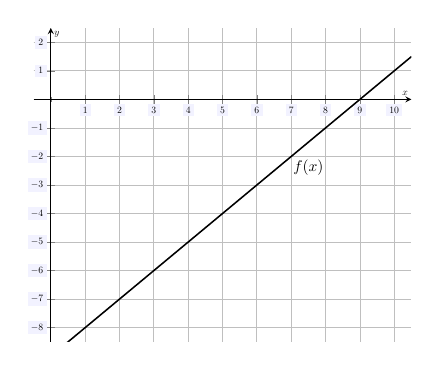
\begin{tikzpicture}[scale=0.7,every node/.style={scale=0.5}]
	\begin{axis}[
	grid=both,
	axis lines=middle,
	ticklabel style={fill=blue!5!white},
	xmin= -0.5, xmax=10.5,
	ymin= -8.5, ymax=2.5,
	xtick={-1,0,...,11},
	ytick={-8,-7,...,2},
	minor tick = {-9,-8,...,3},
	xlabel=\(x\),ylabel=\(y\),
	samples=20]
	\node at (7.5,-2.4) {\scalebox{1.6}{$f(x)$}};
	\addplot[thick, samples=5, domain= -0.5:10.5] {x - 9};
	\end{axis}
	\end{tikzpicture}
	} \hfill
	% Middle
	\fbox{%
	\begin{tikzpicture}[scale=0.7,every node/.style={scale=0.5}]
	\begin{axis}[
	grid=both,
	axis lines=middle,
	ticklabel style={fill=blue!5!white},
	xmin= -0.5, xmax=10.5,
	ymin= -8.5, ymax=2.5,
	xtick={-1,0,...,11},
	ytick={-8,-7,...,2},
	minor tick = {-9,-8,...,3},
	xlabel=\(x\),ylabel=\(y\),
	samples=20]
	\node at (7.5,-3.4) {\scalebox{1.6}{$g(x)$}};
	\addplot[thick, samples=5, domain= -0.5:10.5] {x - 10};
	\addplot[soldot] coordinates{(5,-4)};
	\addplot[holdot] coordinates{(5,-5)};
	\end{axis}
	\end{tikzpicture}
	} \hfill
	% Right
	\fbox{%
	\begin{tikzpicture}[scale=0.7,every node/.style={scale=0.5}]
	\begin{axis}[
	grid=both,
	axis lines=middle,
	ticklabel style={fill=blue!5!white},
	xmin= -0.5, xmax=10.5,
	ymin= -8.5, ymax=2.5,
	xtick={-1,0,...,11},
	ytick={-8,-7,...,2},
	minor tick = {-9,-8,...,3},
	xlabel=\(x\),ylabel=\(y\),
	samples=20]
	\node at (6.5,-2.4) {\scalebox{1.6}{$h(x)$}};
	\addplot[thick, samples=5, domain= -0.5:5] {x - 10};
	\addplot[thick, samples=5, domain= 5:10.5] {x - 8};
	\addplot[soldot] coordinates{(5,-4)};
	\addplot[holdot] coordinates{(5,-3)(5,-5)};
	\end{axis}
	\end{tikzpicture}
	}
	\end{center}
For instance, for the function $f(x)$ on the left, we have $f(5)= -4$ and $\ds\lim_{x \to 5} f(x)= -4$. However, for the function $g(x)$ in the middle, we have $g(5)= -4$ but $\ds\lim_{x \to 5} g(x)= -5$. But for $h(x)$ on the right, we have $h(5)= -4$ but $\ds\lim_{x \to 5} h(x)$ does not exist because the left and right hand limits are not equal. \pvspace{1.3cm}



% 08/26
\checkin{08/26} If $\ds\lim_{x \to a^-} f(x)$ and $\ds\lim_{x \to a^+} f(x)$ exist, then $\ds\lim_{x \to a} f(x)$ exists. \pspace

\sol The statement is \textit{false}. We know that if $\ds\lim_{x \to a} f(x)$ exists, then $\ds\lim_{x \to a^-} f(x)$, exists, $\ds\lim_{x \to a^+} f(x)$ exists, and $\ds\lim_{x \to a^-} f(x)= \lim_{x \to a^+} f(x)$. This is because if $\ds\lim_{x \to a} f(x)$ exists, then $f(x)$ is getting `close' to a single number, say $L$, whenever $x$ is `close' to $a$---no matter if it is `below' or `above' $x= a$. However, just because $f(x)$ is getting `close' to a particular output `on the left' does not mean $f(x)$ is getting `close' to the same output from the right. Take the example from the previous quiz!
	\[
	\fbox{%
	\begin{tikzpicture}[scale=1,every node/.style={scale=0.5}]
	\begin{axis}[
	grid=both,
	axis lines=middle,
	ticklabel style={fill=blue!5!white},
	xmin= -0.5, xmax=10.5,
	ymin= -8.5, ymax=2.5,
	xtick={-1,0,...,11},
	ytick={-8,-7,...,2},
	minor tick = {-9,-8,...,3},
	xlabel=\(x\),ylabel=\(y\),
	samples=20]
	\node at (6.5,-2.4) {\scalebox{1.6}{$h(x)$}};
	\addplot[thick, samples=5, domain= -0.5:5] {x - 10};
	\addplot[thick, samples=5, domain= 5:10.5] {x - 8};
	\addplot[soldot] coordinates{(5,-4)};
	\addplot[holdot] coordinates{(5,-3)(5,-5)};
	\end{axis}
	\end{tikzpicture}
	}
	\]
For this function, we have $\ds\lim_{x \to 5^-} h(x)= -5$, $\ds\lim_{x \to 5^+} h(x)= -3$, but $\ds \lim_{x \to 5^-} h(x) \neq \lim_{x \to 5^+} h(x)$. However, if the left and right hand limits exist \textit{and} are equal, then $\ds\lim_{x \to a} f(x)$ exists.



\newpage



% 08/26
\checkin{08/26} $\ds\lim_{\theta \to 0} \dfrac{\sin(3\theta)}{2\theta}= \dfrac{3}{2}$ \pspace

\sol The statement is \textit{true}. Recall that $\ds\lim_{\Box{} \to 0} \dfrac{\sin(\Box)}{\Box}= 1$. But then\dots
	\[
	\lim_{\theta \to 0} \dfrac{\sin(3\theta)}{2\theta}= \dfrac{1}{2} \lim_{\theta \to 0} \dfrac{\sin(3\theta)}{\theta}= \dfrac{1}{2} \lim_{\theta \to 0} \dfrac{3\sin(3\theta)}{3\theta}= \dfrac{3}{2} \lim_{\theta \to 0} \underbrace{\dfrac{\sin(3\theta)}{3\theta}}_{\squiggle 1}= \dfrac{3}{2} \cdot 1= \dfrac{3}{2}
	\] \pvspace{1.3cm}



% 08/28
\checkin{08/28} $\ds\lim_{x \to 5} \dfrac{x^2 - 3x - 10}{x - 5}= 7$ \pspace

\sol The statement is \textit{true}. We have\dots
	\[
	\lim_{x \to 5} \dfrac{x^2 - 3x - 10}{x - 5}= \lim_{x \to 5} \dfrac{\cancel{(x - 5)}(x + 2)}{\cancel{x - 5}}= \lim_{x \to 5} (x + 2)= 5 + 2= 7
	\] \pvspace{1.3cm}



% 08/29
\checkin{08/29} $\ds \lim_{x \to 1^-} \dfrac{x - 5}{x - 1}= -\infty$ \pspace

\sol The statement is \textit{false}. `Plugging in' $x= 1$, we obtain $\frac{-4}{0}$---so certainly this limit is either $-\infty$, $+\infty$, or DNE. Because we approach $1$ from the left, we know that $x < 1$. But then $x - 1 < 0$. But then $\frac{1}{x - 1}$ approaches $-\infty$ as $x$ tends to 1 from the left. But the numerator is also negative because when $x$ is `close' to 1, $x - 5 < 0$. Therefore, the limit tends to $\infty$. We can see this from the plot of $\frac{x - 5}{x - 1}$. 
	\[
	\fbox{%
	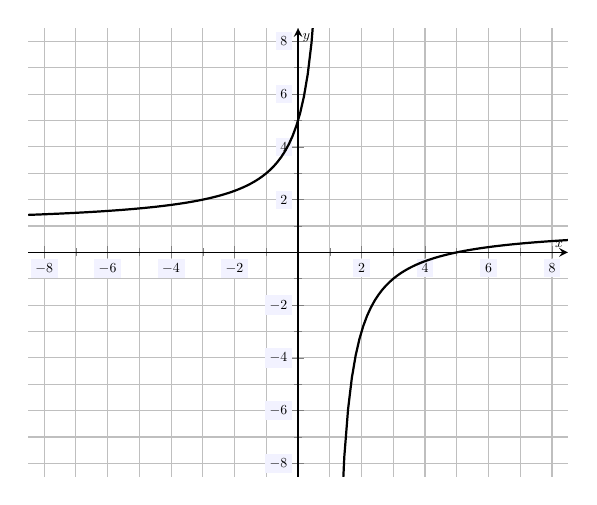
\begin{tikzpicture}[scale=1,every node/.style={scale=0.5}]
	\begin{axis}[
	grid=both,
	axis lines=middle,
	ticklabel style={fill=blue!5!white},
	xmin= -8.5, xmax=8.5,
	ymin= -8.5, ymax=8.5,
	xtick={-10,-8,...,10},
	ytick={-10,-8,...,10},
	minor tick = {-10,-9,...,10},
	xlabel=\(x\),ylabel=\(y\),
	samples=20]
	
	\addplot[thick, samples=80, domain= -8.5:0.9] {(x - 5)/(x - 1)};
	\addplot[thick, samples=80, domain= 1.1:10.5] {(x - 5)/(x - 1)};
	
	\end{axis}
	\end{tikzpicture}
	}
	\]
The given answer failed to take the sign of the numerator into account. 



\newpage



% 09/04
\checkin{09/04} $\ds \lim_{x \to \infty} \dfrac{9x^2 - 5x + 7}{8 - 3x^2}= 3$ \pspace

\sol The statement is \textit{true}. We know that $\ds\lim_{x \to \pm \infty} \dfrac{\text{polynomial}}{\text{polynomial}}$ is 0 if $\deg \text{ den.} > \deg \text{ num.}$, $\pm \infty$ (depending on the limit and sign of the leading coefficient in the numerator) if $\deg \text{ num.} > \deg \text{ den.}$, and is the ratio of the leading coefficients if $\deg \text{ den.}= \deg \text{ num.}$. The degree of the numerator and denominator is 2. Therefore, we know that 
	\[
	\lim_{x \to \infty} \dfrac{9x^2 - 5x + 7}{8 - 3x^2}= \dfrac{9}{-3}= -3
	\]
The given answer did not correctly identify the leading coefficient in the denominator. Alternatively, we can multiply by $\frac{1/x^{\deg \text{ denom}}}{1/x^{\deg \text{ denom}}}$:
	\[
	\lim_{x \to \infty} \dfrac{9x^2 - 5x + 7}{8 - 3x^2}= \lim_{x \to \infty} \dfrac{9x^2 - 5x + 7}{8 - 3x^2} \cdot \dfrac{1/x^2}{1/x^2}= \lim_{x \to \infty} \dfrac{9 - \frac{5}{x} + \frac{7}{x}}{\frac{8}{x^2} - 3}= \dfrac{9 - 0 + 0}{0 - 3}= \dfrac{9}{-3}= -3
	\] \pvspace{1.3cm}



% 09/05
\checkin{09/05} If $f(x)$ is defined to be the following function: 
	\[
	f(x)= 
	\begin{cases}
	x^2 + x - 6, & x < -1 \\
	x - 5, & x \geq -1 
	\end{cases}
	\]
Then $f(x)$ is everywhere continuous. \pspace

\sol The statement is \textit{true}. If $x < -1$, then $f(x)= x^2 + x - 6$. We know that $x^2 + x - 6$ is a polynomial, which are everywhere continuous. If $x > -1$, then $f(x)= x - 5$, which is a polynomial. We know that polynomials are everywhere continuous. Therefore, we know $f(x)$ is continuous when $x < -1$ and when $x > -1$. We only need to check if $f(x)$ is continuous at $x= -1$. For $f(x)$ to be continuous at $x= -1$, we need to check that $\ds f(-1)= \lim_{x \to -1} f(x)$:
	\begin{itemize}
	\item $f(-1)= -1 - 5= -6$
	\item $\ds\lim_{x \to -1^-} f(x)= \lim_{x \to -1^-} (x^2 + x - 6)= (-1)^2 + (-1) - 6= -6$
	\item $\ds\lim_{x \to -1^+} f(x)= \lim_{x \to -1^+} (x - 5)= -1 - 5= -6$
	\end{itemize}
Because $\ds\lim_{x \to -1^-} f(x)= \ds\lim_{x \to -1^+} f(x)$, we know that $\ds\lim_{x \to -1} f(x)= -6$. Therefore, $\ds f(-1)= \lim_{x \to -1} f(x)$. But then $f(x)$ is continuous at $x= -1$. Therefore, $f(x)$ is continuous for all $x$, i.e. $f(x)$ is everywhere continuous. 



\newpage



% 09/09
\checkin{09/09} The function $f(x)= |xe^x \sin x|$ is continuous. Therefore, $\ds\lim_{x \to \pi} f(x)= f \left( \lim_{x \to \pi} \right)= f(\pi)= 0$. \pspace

\sol The statement is \textit{true}. We know that $x$, $e^x$, and $\sin x$ are everywhere continuous. Therefore, their product---$g(x):= x e^x \sin x$---is continuous. We also know the function $h(x)= |x|$ is everywhere continuous. But then the composition $(h \circ g)(x)$ is continuous. But $(h \circ g)(x)= h \big( g(x) \big)= h(x e^x \sin x)= |xe^x \sin x|$. 
We can see the continuity from a plot of this function. 
	\[
	\fbox{%
	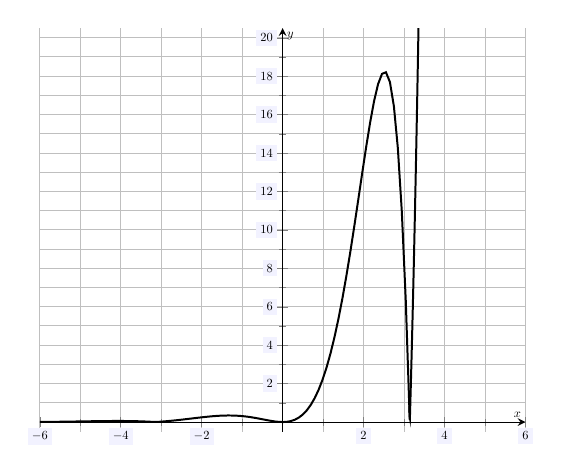
\begin{tikzpicture}[scale=0.9,every node/.style={scale=0.5}]
	\begin{axis}[
	grid=both,
	axis lines=middle,
	ticklabel style={fill=blue!5!white},
	xmin= -6, xmax=6,
	ymin= -0.5, ymax=20.5,
	xtick={-6,-4,...,6},
	ytick={-2,0,...,20},
	minor tick = {-6,-5,...,0,1,2,...,20},
	xlabel=\(x\),ylabel=\(y\),
	samples=20]
	
	\addplot[thick, samples=120, domain= -8.5:3.14] {abs(x*2.71828^x*sin(deg(x)))};
	\addplot[thick, samples=120, domain= 3.13:4] {abs(x*2.71828^x*sin(deg(x)))};
	
	\end{axis}
	\end{tikzpicture}
	}
	\]
Finally, we know that if a function $f(x)$ is continuous at $x= a$, then $\ds \lim_{x \to a} f(x)= f(a)$. But we know that the given $f(x)$ is continuous at $x= \pi$---it is everywhere continuous. But then\dots
	\[
	f(\pi)= |\pi \cdot e^\pi \sin \pi|= |\pi \cdot e^\pi \cdot 0|= |0|= 0
	\] \pvspace{1.3cm}



% 09/10
\checkin{09/10} The function $f(x)$, plotted below, is \textit{not} differentiable at $x= -2$ but \textit{is differentiable} at $x= 6$.
	\[
	\fbox{
	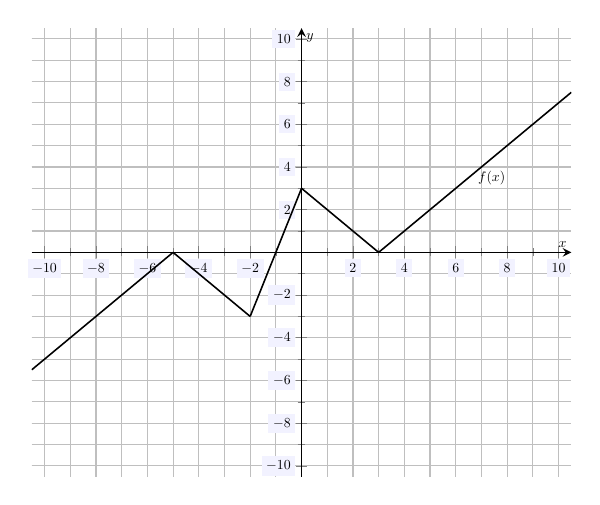
\begin{tikzpicture}[scale=1,every node/.style={scale=0.5}]
	\begin{axis}[
	grid=both,
	axis lines=middle,
	ticklabel style={fill=blue!5!white},
	xmin= -10.5, xmax=10.5,
	ymin= -10.5, ymax=10.5,
	xtick={-10,-8,-6,-4,-2,0,2,4,6,8,10},
	ytick={-10,-8,-6,-4,-2,0,2,4,6,8,10},
	minor tick = {-10,-9,...,10},
	xlabel=\(x\),ylabel=\(y\),
	]
	\node at (7.4,3.5) {$f(x)$};
	\addplot[line width= 0.02cm,samples=200,domain= 0:10.5] ({x},{abs(x-3)});
	\addplot[line width= 0.02cm,samples=200,domain= -10.5:-2] ({x},{-1*abs(x+5)});
	\addplot[line width= 0.02cm,samples=200,domain= -2:0] ({x},{3+3*x});
	\end{axis}
	\end{tikzpicture}
	}
	\] 

\sol The statement is \textit{true}. At $x= -2$, we can see that $f(x)$ has a cusp. [The derivative somehow `wants' to be $-1$ and 3 at the same time.] Therefore, $f(x)$ is not differentiable at $x= -2$. However, we can see that $f(x)$ is linear at $x= 6$. We know linear functions are differentiable---the derivative is the slope of the function. Therefore, $f(x)$ is differentiable at $x= 6$. In fact, the value of the derivative at $x= 6$ is the slope of the line through $\big(6, f(x) \big)$---which is $3x + 3$ so that $f'(6)= 3$. 



\newpage



% 09/11
\checkin{09/11} \textit{Every} differentiable function is continuous, but not every continuous function is differentiable. \pspace

\sol The statement is \textit{true}. We know that every differentiable function is continuous. However, not every continuous function is necessarily differentiable. For instance, consider the function $f(x)= |x|$, shown below.
	\[
	\fbox{
	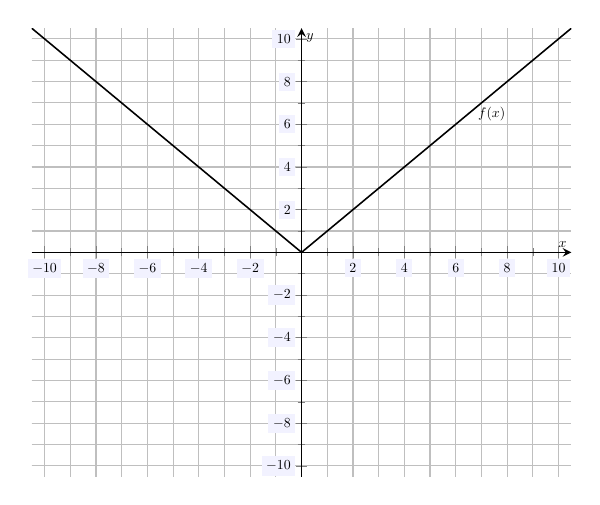
\begin{tikzpicture}[scale=1,every node/.style={scale=0.5}]
	\begin{axis}[
	grid=both,
	axis lines=middle,
	ticklabel style={fill=blue!5!white},
	xmin= -10.5, xmax=10.5,
	ymin= -10.5, ymax=10.5,
	xtick={-10,-8,-6,-4,-2,0,2,4,6,8,10},
	ytick={-10,-8,-6,-4,-2,0,2,4,6,8,10},
	minor tick = {-10,-9,...,10},
	xlabel=\(x\),ylabel=\(y\),
	]
	\node at (7.4,6.5) {$f(x)$};
	\addplot[line width= 0.02cm,samples=3,domain= -10.5:10.5] ({x},{abs(x)});
	\end{axis}
	\end{tikzpicture}
	}
	\] 
We see that $f(x)$ has a cusp at $x= 0$. Therefore, $f(x)$ is not differentiable at $x= 0$. We can check this directly:
	\[
	f'(0):= \lim_{h \to 0} \dfrac{f(0 + h) - f(0)}{h}= \dfrac{|h| - 0}{h}= \begin{cases} \dfrac{h}{h}= 1, h > 0 \\ \\\dfrac{-h}{h}= -1, & h < 0 \end{cases}
	\]
This limit does not exist. Therefore, $f'(0)$ does not exist. There are other functions, e.g. the Weierstrass function shown below, that are \textit{everywhere} continuous but \textit{nowhere} differentiable. 

	\begin{figure}[!ht]
	\centering
	\fbox{%
	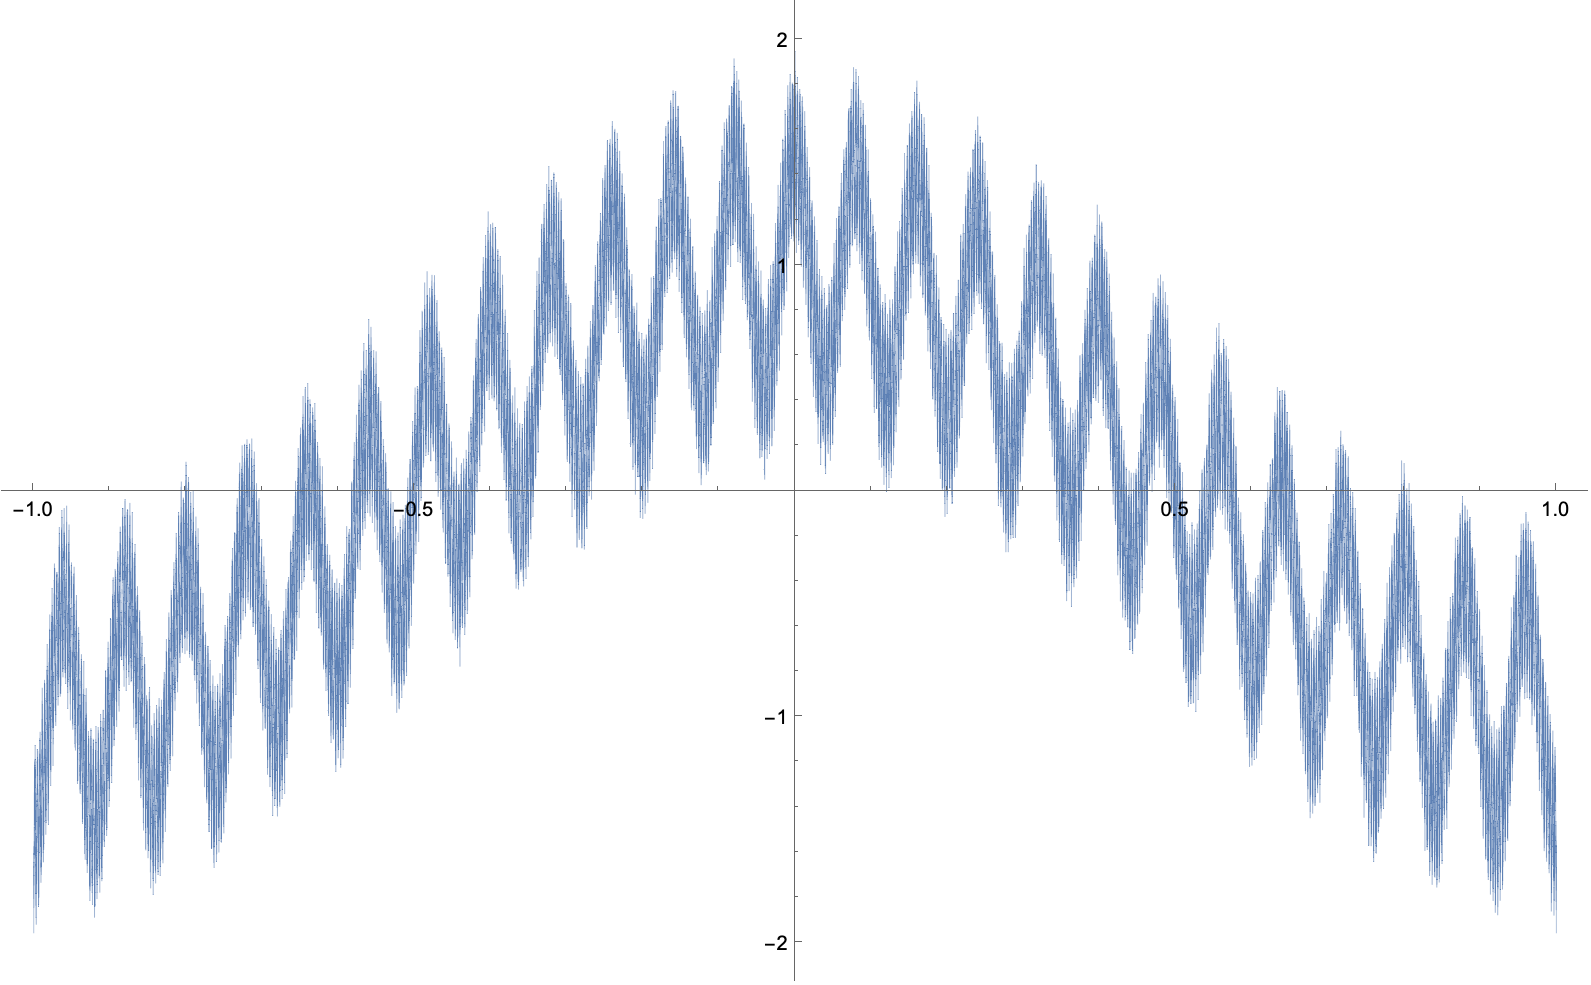
\includegraphics[width=0.5\textwidth]{weierstrass.png}
	}
	\end{figure} \pvspace{1.3cm}



\newpage



% 09/12
\checkin{09/12} $\ds \dfrac{d}{dx} \left( e^{-x} \cos x \right)= -e^{-x} \cos x - e^{-x} \sin x$ \pspace

\sol The statement is \textit{true}. We use the product rule and the chain rule. We have\dots
	\[
	\begin{aligned}
	\dfrac{d}{dx} \left( e^{-x} \cos x \right)&= \dfrac{d}{dx} (e^{-x}) \cos x + e^{-x} \dfrac{d}{dx} ( \cos x) \\[0.3cm]
	&= (-e^{-x}) \cos x + e^{-x} (-\sin x) \\[0.3cm]
	&= -e^{-x} \cos x - e^{-x} \sin x \\[0.3cm]
	&= -e^{-x} (\sin x + \cos x)
	\end{aligned}
	\] \pvspace{1cm}



% 09/16
\checkin{09/16} $\ds \dfrac{d}{dx} \left(x 3^x \right)^{10}= 10 \left(3^x + x3^x \right)^9$ \pspace

\sol The statement is \textit{false}. The chain rule has not been properly applied. The individual began to apply the chain rule by beginning with the power rule---but then let the base be result of the next step in the chain rule---while also incorrectly taking the derivative of $3^x$. [The derivative of $b^x$ is $b^x \ln b$.] We have\dots
	\[
	\dfrac{d}{dx} \left(x 3^x \right)^{10}= 10 \left(x 3^x \right)^9 \cdot \dfrac{d}{dx} \left(x 3^x \right)= 10(x3^x) \cdot (3^x + x 3^x \ln 3)
	\]
Of course, one could perform some arithmetic first to avoid the chain rule---mostly:
	\[
	\dfrac{d}{dx} \left(x 3^x \right)^{10}= \dfrac{d}{dx} x^10 3^{10x}= 10x^9 \cdot 3^{10x} + x^{10} \cdot \left( 3^{10x} \ln 3 \cdot 10 \right)
	\] \pvspace{1.3cm}



% 09/18
\checkin{09/18} $\dfrac{d}{dx} \left( \dfrac{f}{g} \right)= \dfrac{f' g - g' f}{g^2}$ \pspace

\sol The statement is \textit{true}. This is the quotient rule! Indeed, we can derive this using the power and chain rules:
	\[
	\dfrac{d}{dx} \left( \dfrac{f}{g} \right)= \dfrac{d}{dx} \left( f \cdot (g)^{-1} \right)= f' \cdot (g)^{-1} + f \cdot (- g^{-2} \cdot g')= \dfrac{f'}{g} - \dfrac{fg'}{g^2}= \dfrac{f' g}{g^2} - \dfrac{f g'}{g^2}= \dfrac{f' g - f g'}{g^2}
	\] \pvspace{1.3cm}



% 09/19
\checkin{09/19} Let $f(x)$ be a twice-differentiable function. If $f'(x) > 0$, then it must be that $f''(x) > 0$. \pspace

\sol The statement is \textit{false}. Recall that if $f'(x) > 0$, the function $f(x)$ is increasing at that $x$-value, and if $f'(x) < 0$, the function $f(x)$ is decreasing at that $x$-value. Furthermore, recall that if $f''(x) > 0$, the function $f(x)$ is concave up at that $x$-value, and if $f''(x) < 0$, the function $f(x)$ is concave down at that $x$-value. Therefore, the question is asking if a function is increasing, does it have to be concave up. This is certainly not the case. For instance, consider the function $f(x)$ shown below. 
	\[
	\fbox{
	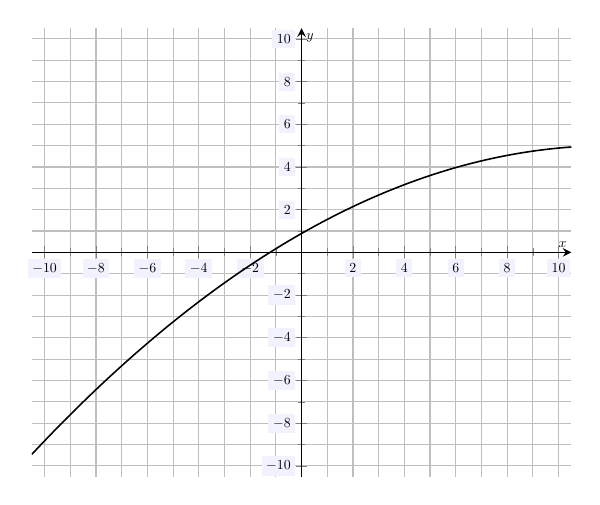
\begin{tikzpicture}[scale=1,every node/.style={scale=0.5}]
	\begin{axis}[
	grid=both,
	axis lines=middle,
	ticklabel style={fill=blue!5!white},
	xmin= -10.5, xmax=10.5,
	ymin= -10.5, ymax=10.5,
	xtick={-10,-8,-6,-4,-2,0,2,4,6,8,10},
	ytick={-10,-8,-6,-4,-2,0,2,4,6,8,10},
	minor tick = {-10,-9,...,10},
	xlabel=\(x\),ylabel=\(y\),
	]
	\addplot[line width= 0.02cm,samples=100,domain= -10.5:10.5] ({x},{5 - 1/35*(x - 12)^2});
	\end{axis}
	\end{tikzpicture}
	}
	\] 
This function is clearly everywhere increasing, so that $f'(x) > 0$. However, observe that the function is concave down, so that $f''(x) < 0$. The sign of $f'$ and $f''$ do indeed give you information about $f(x)$. However, the signs of $f$, $f'$, and $f''$ \textit{do not} need to be the same. \pvspace{1.3cm}



% 10/07
\checkin{10/07} $\dfrac{d}{dx} \left( x^2 + y^2 - \sin^2(xy) \right)= 2x + 2yy' - \cos^2(xy)  (y + x)$ \pspace

\sol The statement is \textit{false}. This is implicit differentiation. One must remember that $\dfrac{d}{dx}\, y= y'$---and to properly apply derivative rules:
	\[
	\dfrac{d}{dx} \left( x^2 + y^2 - \sin^2(xy) \right)= 2x + 2y\, \dfrac{dy}{dx} - 2 \sin(xy) \cdot \cos(xy) \cdot \left(1 \cdot y + x \cdot \dfrac{dy}{dx} \right)
	\] \pvspace{1.3cm}



% 10/07
\checkin{10/07} Suppose that $f'(a)= 0$ and $f(x)$ has a local maximum at $x= a$. Then $f'(x)$ changes sign at $x= a$ and $f''(a) < 0$. \pspace

\sol The statement is \textit{false}. We know that $f'(a)= 0$, i.e. $x= a$ is a critical value, and $f(x)$ has a local maximum at $x= a$. Because the first derivative test applies, it must be that $f'(x)$ changes sign at $x= a$---from positive to negative across $x= a$. We can also determine that $x= a$ is a local maxima by the second derivative test if $f''(a) < 0$. However, if $x= a$ is a local maxima, the second derivative test may not apply. For instance, the function may not be twice differentiable---even if it is differentiable. Furthermore, it could be that $f''(a)= 0$---so that the second derivative test is inconclusive. For instance, consider the function $f(x)= 1 - x^4$ and take $a= 0$. We have $f'(x)= -4x^3$ so that $f'(0)= 0$. We know that $f'(-0.1) > 0$ and $f'(0.1) < 0$, i.e. $f'(x)$ changes sign from positive to negative. Therefore, $x= 0$ is a local maximum, which we can see in the plot below. However, $f''(x)= -12x^2$ and $f''(0)= 0$. Therefore, the second derivative test is inconclusive. 
	\[
	\fbox{
	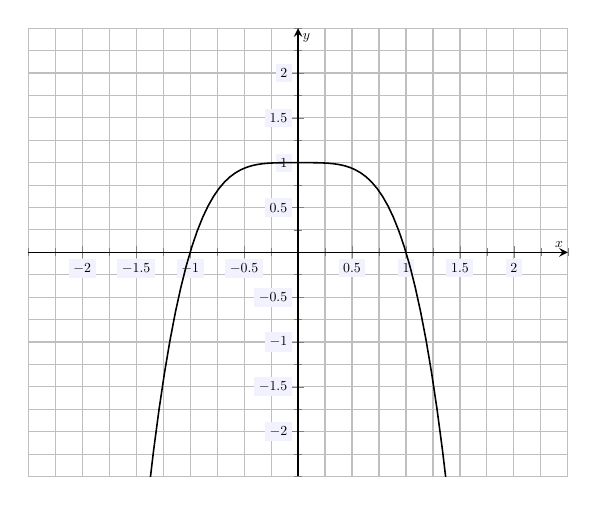
\begin{tikzpicture}[scale=1,every node/.style={scale=0.5}]
	\begin{axis}[
	grid=both,
	axis lines=middle,
	ticklabel style={fill=blue!5!white},
	xmin= -2.5, xmax=2.5,
	ymin= -2.5, ymax=2.5,
	xtick={-2,-1.5,...,2},
	ytick={-2,-1.5,...,2},
	minor tick = {-2.5,-2.25,...,2.5},
	xlabel=\(x\),ylabel=\(y\),
	]
	\addplot[line width= 0.02cm,samples=100,domain= -2.5:2.5] ({x},{1 - x^4});
	\end{axis}
	\end{tikzpicture}
	}
	\] \pvspace{1.3cm}



% 10/14
\checkin{10/14} A function can have infinitely many local maxima or local minima. \pspace

\sol The statement is \textit{true}. Consider the function $f(\theta)= \cos(\theta)$, plotted below. 
	\[
	\fbox{
	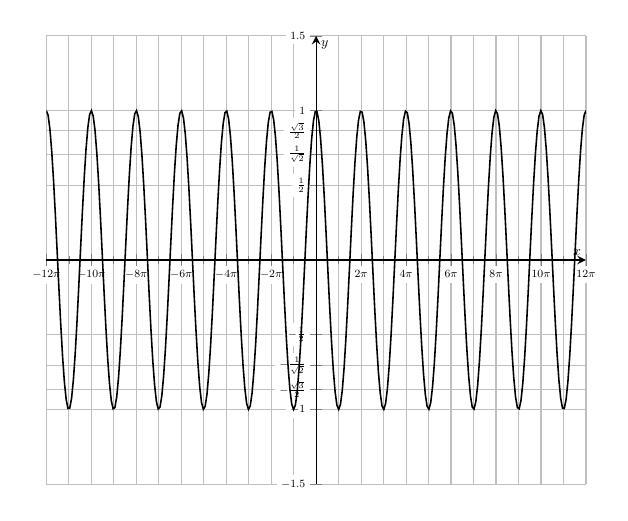
\begin{tikzpicture}[scale=1,every node/.style={scale=0.5}]
	\begin{axis}[
	grid=both,
	axis lines=middle,
	ticklabel style={fill=blue!5!white},
	xmin= -12*pi, xmax=12*pi,
	ymin= -1.5, ymax=1.5,
	xtick={-12*pi,-10*pi,...,12*pi},
	ytick={-1.5,-1,-sqrt(3)/2,-1/sqrt(2),-1/2,0,1/2,1/sqrt(2),sqrt(3)/2,1,1.5},
	xticklabel style={font=\footnotesize,fill=white},
	xticklabels={$-12\pi$,$-10\pi$,$-8\pi$,$-6\pi$,$-4\pi$,$-2\pi$,$0$,$2\pi$,$4\pi$,$6\pi$,$8\pi$,$10\pi$,$12\pi$},
	yticklabel style={font=\footnotesize,fill=white},
	yticklabels={$-1.5$,$-1$,$-\frac{\sqrt{3}}{2}$,$-\frac{1}{\sqrt{2}}$,$-\frac{1}{2}$,$0$,$\frac{1}{2}$,$\frac{1}{\sqrt{2}}$,$\frac{\sqrt{3}}{2}$,$1$,$1.5$},
	minor tick = {-12*pi,-11*pi,...,12*pi},
	xlabel=\(x\),ylabel=\(y\),
	]
	\addplot[line width= 0.02cm,samples=300,domain= -12*pi:12*pi] ({x},{cos(deg(x))});
	\end{axis}
	\end{tikzpicture}
	}
	\]
We know that $f(\theta)= \cos(\theta)$ has a local maxima at each even integer multiple of $\pi$ and local minima at each odd integer multiple of $\pi$. In fact, a function can have infinitely many local maxima/minima on a finite interval. Consider the function $f(x)= \cos\left( \frac{1}{x} \right)$ for $0 < x \leq 1$ and $f(0)= 1$ if $x= 0$. This function has infinitely many local maxima and minima on $[0, 1]$. For instance, it has a local maxima whenever $x= \frac{1}{2k \pi}$ for any integer $k > 0$ and a local minima whenever $x= \frac{1}{(2k + 1) \pi}$ for any integer $k > 0$. \par
	\[
	\fbox{
	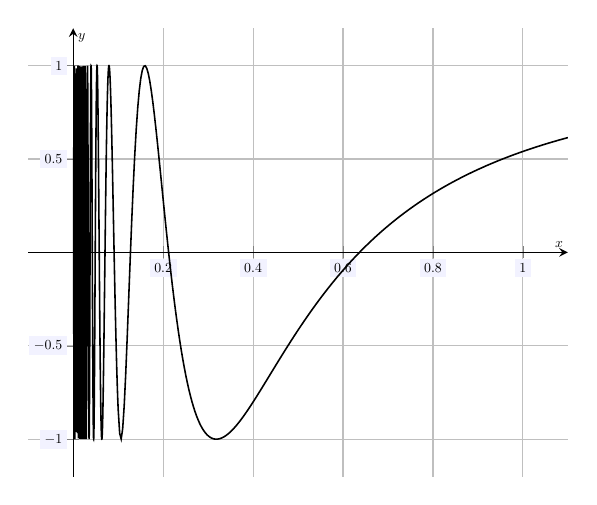
\begin{tikzpicture}[scale=1,every node/.style={scale=0.5}]
	\begin{axis}[
	grid=both,
	axis lines=middle,
	ticklabel style={fill=blue!5!white},
	xmin= -0.1, xmax=1.1,
	ymin= -1.2, ymax=1.2,
	xlabel=\(x\),ylabel=\(y\),
	]
	\addplot[line width= 0.02cm,samples=1000,domain= 0.001:0.1] ({x},{cos((1/x)r)});
	\addplot[line width= 0.02cm,samples=300,domain= 0.1:1.1] ({x},{cos((1/x)r)});
	\end{axis}
	\end{tikzpicture}
	}
	\] \pvspace{1.3cm}



% 10/15
\checkin{10/15} The \textit{Froude number}, $F_r$, is a dimensionless value that is used in the description of open channel flows. Specifically, it is the ratio of inertial and gravitational forces. Using this, we have $F_r= \dfrac{v}{\sqrt{gD}}$, where $v$ is the water velocity, $D$ is the hydraulic depth, and $g$ is the constant gravitational attraction. Given this, their rates of changes with respect to time are related by\dots
	\[
	\dfrac{dF_r}{dt}= \dfrac{\frac{dv}{dt}\, \sqrt{gD} - v \, \frac{\sqrt{g}}{2 \sqrt{D}}\, \frac{dD}{dt}}{gD}
	\] \pspace

\sol The statement is \textit{true}. Implicitly differentiating with respect to $t$, we have\dots
	\[
	\begin{gathered}
	F_r= \dfrac{v}{\sqrt{gD}} \\
	\dfrac{d}{dt} \,F_r= \dfrac{d}{dt} \left( \dfrac{v}{\sqrt{gD}} \right) \\
	\dfrac{dF_r}{dt}= \dfrac{\dfrac{d}{dt}\, v \cdot \sqrt{gD} - \dfrac{d}{dt} ( \sqrt{g} \sqrt{D}) \cdot v}{\sqrt{gD}^2} \\
	\dfrac{dF_r}{dt}= \dfrac{\dfrac{dv}{dt}\, \sqrt{gD} - \left( \sqrt{g}\, \dfrac{D'}{2\sqrt{D}} \right) \cdot v}{gD} \\
	\dfrac{dF_r}{dt}= \dfrac{\frac{dv}{dt}\, \sqrt{gD} - v \, \frac{\sqrt{g}}{2 \sqrt{D}}\, \frac{dD}{dt}}{gD}
	\end{gathered}
	\]



\newpage



% 10/16
\checkin{10/16} If one wants to find the rate of change of the distance between two objects, one at $\big(x_1(t), y_1(t) \big)$ and the other at $\big(x_2(t), y_2(t) \big)$, then one can implicitly differentiation $d^2= (x_1 - x_2)^2 + (y_1 - y_2)^2$ with respect to time, $t$. \pspace

\sol The statement is \textit{true}. The distance between the objects at time $t$ is given by\dots
	\[
	d= \sqrt{ \big(x_1(t) - x_2(t) \big)^2 + \big(y_1(t) - y_2(t) \big)^2}
	\]
One can then implicitly differentiate with respect to time, $t$, to find the rate of change in the distance between the objects. 
	\[
	\begin{aligned}
	d&= \sqrt{ \big(x_1(t) - x_2(t) \big)^2 + \big(y_1(t) - y_2(t) \big)^2} \\[0.2cm]
	\dfrac{d}{dt} \, d&= \dfrac{d}{dt}\, \sqrt{ \big(x_1(t) - x_2(t) \big)^2 + \big(y_1(t) - y_2(t) \big)^2} \\[0.2cm]
	d'&= \frac{1}{2} \left( \big(x_1(t) - x_2(t) \big)^2 + \big(y_1(t) - y_2(t) \big)^2 \right)^{-1/2} \cdot \\[0.2cm]
	\phantom{d'}&\phantom{= -----} \left( 2 \big(x_1(t) - x_2(t) \big) \cdot \big(x_1'(t) - x_2'(t) \big) + 2 \big( y_1(t) - y_2(t) \big) \cdot \big( y_1'(t) - y_2'(t) \big) \right)  \\[0.2cm]
	d'&= \dfrac{\big(x_1(t) - x_2(t) \big) \cdot \big(x_1'(t) - x_2'(t) \big) + \big( y_1(t) - y_2(t) \big) \cdot \big( y_1'(t) - y_2'(t) \big)}{\sqrt{\big(x_1(t) - x_2(t) \big)^2 + \big(y_1(t) - y_2(t) \big)^2}}
	\end{aligned}
	\]
Alternatively, we can square to avoid the square root and then implicitly differentiate: 
	\[
	\begin{aligned}
	d&= \sqrt{ \big(x_1(t) - x_2(t) \big)^2 + \big(y_1(t) - y_2(t) \big)^2} \\[0.2cm]
	d^2&= \big(x_1(t) - x_2(t) \big)^2 + \big(y_1(t) - y_2(t) \big)^2 \\[0.2cm]
	\dfrac{d}{dt}\, d^2 &= \dfrac{d}{dt}\, \big(x_1(t) - x_2(t) \big)^2 + \big(y_1(t) - y_2(t) \big)^2 \\[0.2cm]
	2d \cdot d' &= 2 \big(x_1(t) - x_2(t) \big) \cdot \big(x_1'(t) - x_2'(t) \big) + 2 \big(y_1(t) - y_2(t) \big) \cdot \big(y_1'(t) - y_2'(t) \big) \\[0.2cm]
	d' &= \dfrac{\big(x_1(t) - x_2(t) \big) \cdot \big(x_1'(t) - x_2'(t) \big) + \big(y_1(t) - y_2(t) \big) \cdot \big(y_1'(t) - y_2'(t) \big)}{d} \\[0.2cm]
	d' &= \dfrac{\big(x_1(t) - x_2(t) \big) \cdot \big(x_1'(t) - x_2'(t) \big) + \big(y_1(t) - y_2(t) \big) \cdot \big(y_1'(t) - y_2'(t) \big)}{\sqrt{ \big(x_1(t) - x_2(t) \big)^2 + \big(y_1(t) - y_2(t) \big)^2}}
	\end{aligned}
	\] \pvspace{1.3cm}



% 10/21
\checkin{10/21} If $f(x)$ is a continuous function with $f(1)= 1$ and $f(5)= 4$, then there is an $x \in [1, 5]$ with $f(x)^2 + 4= 10$.  \pspace

\sol The statement is \textit{true}. Because $f(x)$ is continuous, we know that $f(x)^2$ is continuous---being the product of continuous functions. Now $f(1)^2= 1^2= 1$ and $f(5)^2= 4^2= 16$. Observe that $f(x)^2 + 4= 10$ has a solution if and only if $f(x)^2= 6$. But $f(1)^2= 1 < 6 < 16= f(5)^2$. Therefore, by the Intermediate Value Theorem, there is a $c \in [1, 5]$ such that $f(c)^2= 6$. But then $f(c)^2 + 4= 6 + 4= 10$, i.e. there is a solution to $f(x)^2 + 4= 10$ on $[1, 5]$. 



\newpage



% 10/30
\checkin{10/30} $\ds\int_{-1}^1 \sqrt{1 - x^2} \,dx= \frac{\pi}{2}$  \pspace

\sol The statement is \textit{true}. Let $y= \sqrt{1 - x^2}$. We want to compute $\ds\int_{-1}^1 \sqrt{1 - x^2} \,dx= \int_{-1}^1 y(x) \,dx$. But if $y= \sqrt{1 - x^2}$, then $y^2= 1 - x^2$, which implies that $x^2 + y^2= 1$. But this is the circle with radius 1 centered at the origin. This shows us that $y= \sqrt{1 - x^2}$ on $[-1, 1]$ is the `upper half' of this unit circle. We know that $\ds\int_{-1}^1 \sqrt{1 - x^2} \,dx$ is the (signed) area between the curve and the $x$-axis. We know that the area of a circle is $\pi r^2$. For the whole unit circle, $A= \pi r^2= \pi (1^2)= \pi$. But then the area of the half circle is $\frac{\pi}{2}$. Therefore, $\ds\int_{-1}^1 \sqrt{1 - x^2} \,dx= \frac{\pi}{2}$. \pvspace{1.3cm}



% 11/04
\checkin{11/04} Both $\sin^2 x$ and $-\frac{1}{2} \cos(2x)$ are antiderivatives for $\sin(2x)$, i.e. they are solutions to $\ds\int \sin(2x) \,dx$. \pspace

\sol The statement is \textit{true}. Recall that an antiderivative (if it exists) for a function $f(x)$ is a function $F(x)$ such that $F'(x)= f(x)$. Observe that\dots
	\[
	\begin{aligned}
	\dfrac{d}{dx} \, \sin^2 x&= 2 \sin x \cdot \cos x= \sin(2x) \\[0.3cm]
	\dfrac{d}{dx} \, -\frac{1}{2}\, \cos(2x)&= -\dfrac{1}{2}\, \cdot -\sin(2x) \cdot 2= \sin(2x)
	\end{aligned}
	\]
Therefore, these are both antiderivatives of $\sin(2x)$, i.e. solutions to $\ds\int \sin(2x) \,dx$. For the most general form of a antiderivative for $\sin(2x)$ is $\ds\int \sin(2x) \,dx= -\dfrac{\cos(2x)}{2} + C$. Observe that this also shows there is some $C$ such that $-\frac{1}{2} \cos(2x) + C= \sin^2 x$. Recalling that $\sin^2 x= \frac{1 - \cos(2x)}{2}$, we see that $C= \frac{1}{2}$. One can also substitute any $x$ value and then solve for $C$ to find that $C= \frac{1}{2}$. \pvspace{1.3cm}



% 11/06
\checkin{11/06} $\ds \dfrac{d}{dx} \int_{\sin x}^9 e^{t^3} \;dt= 3x^2 e^{\sin^3 x} + C$ \pspace

\sol The statement is \textit{false}. Recall that from the Second Fundamental Theorem of Calculus, we have\dots
	\[
	\dfrac{d}{dx} \int_c^{g(x)} f(t) \,dt= f \big(g(x) \big) \cdot g'(x)
	\]
But observe that the \textit{lower limit} is the constant and one differentiates the upper limit---not the integrant. Moreover, there is never a `$+ C$' in these problems. We must first rewrite the integral and then properly apply the theorem:
	\[
	 \dfrac{d}{dx} \int_{\sin x}^9 e^{t^3} \;dt= - \dfrac{d}{dx} \int_9^{\sin x} e^{t^3} \;dt= -e^{\sin^3 x} \cdot \dfrac{d}{dx} \, (\sin x)= -e^{\sin^3 x} \cos x 
	\]



\newpage



% 11/11
\checkin{11/11} The area bound by the curves $y= x^3$ and $y= x$ is given by $\ds\int_{-1}^1 (x^3 - x) \; dx$. \pspace

\sol The statement is \textit{false}. Recall that when we say the area bound by curves, we mean that to be the \textit{area} not the \textit{signed/directed area}; that is, the area bound by curves must be zero or bigger, i.e. nonnegative. We first find the intersection of these curves. If $x^3= x$, then $x^3 - x= 0$. But $x^3 - x= x(x^2 - 1)= x(x - 1)(x + 1)$. Therefore, the solutions are $x= -1$, $x= 0$, and $x= 1$. If one na\"ively integrates, we find that $\ds\int_{-1}^1 (x^3 - x) \; dx= 0$. But yet, we can see on the plot below that there is indeed area between them! 
	\[
	\fbox{
	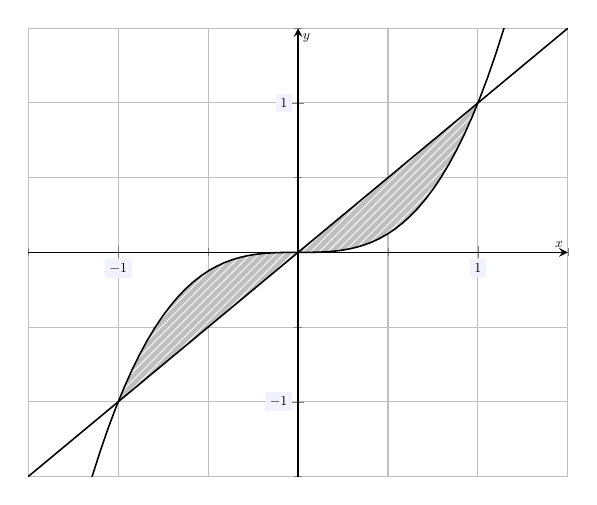
\begin{tikzpicture}[scale=1,every node/.style={scale=0.5}]
	\begin{axis}[
	grid=both,
	axis lines=middle,
	ticklabel style={fill=blue!5!white},
	xmin= -1.5, xmax=1.5,
	ymin= -1.5, ymax=1.5,
	xtick={-2,-1,...,2},
	ytick={-2,-1,...,2},
	minor tick = {-2.5,-2,...,2.5},
	xlabel=\(x\),ylabel=\(y\),
	]
	\addplot[name path= F, line width= 0.02cm,samples=80,domain= -1.7:1.7] ({x},{x^3 });
	\addplot[name path= G, line width= 0.02cm,samples=10,domain= -3.6:3.5] ({x},{x});
	
	\addplot[color=gray!50] fill between[of= F and G, soft clip={domain= -1:1}];
	\addplot[pattern= north east lines, pattern color=gray!10] fill between[of=F and G, soft clip={domain= -1:1}];
	\end{axis}
	\end{tikzpicture}
	}
	\]
The issue is that some of this area was treated as negative because the area was not computed properly. To make sure that the area is treated as `positive', we need to be sure that we integrate the `top' curve minus the `bottom' curve. But which is the `top' flips across this region. On $[-1, 0]$, $y= x^3$ is the `top' curve, while on $[0, 1]$, $y= x$ is the `top' curve. Therefore, to compute the area correctly, we need to compute the following:
	\[
	\begin{gathered}
	A= \int_{-1}^0 (x^3 - x) \;dx + \int_0^1 (x - x^3) \;dx \\[0.3cm]
	A= \left( \frac{1}{4}\, x^4 - \frac{1}{2}\, x^2 \right) \bigg|_{-1}^0 + \left( \frac{1}{2}\, x^2 - \frac{1}{4}\, x^4 \right) \bigg|_0^1 \\[0.3cm]
	A= \left[ \left( 0 - 0 \right) - \left( \dfrac{1}{4} - \dfrac{1}{2} \right) \right] + \left[ \left( \dfrac{1}{2} - \dfrac{1}{4} \right) - \left( 0 - 0 \right) \right] \\[0.3cm]
	A= \left[ 0 - \left(- \dfrac{1}{4} \right) \right] + \left[ \dfrac{1}{4} - 0 \right] \\[0.3cm]
	A= \dfrac{1}{4} + \dfrac{1}{4} \\[0.3cm]
	A= \dfrac{1}{2}
	\end{gathered}
	\] \pvspace{1.3cm}



\newpage



% 11/13
\checkin{11/3} The substitution $u= \sqrt{x}$ allows one to write the integral $\ds\int\sqrt{x} \, e^{\sqrt{x}}\;dx$ as $\ds\frac{1}{2} \int e^u \;du$. Therefore, $\ds\int \sqrt{x} \, e^{\sqrt{x}} \;dx= \frac{1}{2}\, e^{\sqrt{x}} + C$. \pspace

\sol The statement is \textit{false}. If this were the case, then $\dfrac{d}{dx} \,(\frac{1}{2}\, e^{\sqrt{x}} + C)= \frac{1}{2}\, e^{\sqrt{x}} \cdot \frac{1}{2 \sqrt{x}} = \frac{e^{\sqrt{x}}}{4 \sqrt{x}} \neq \sqrt{x} \, e^{\sqrt{x}}$. Observe that if one chooses $u= \sqrt{x}$, then $du= \frac{1}{2\sqrt{x}} \,dx$. But then $dx= 2 \sqrt{x} \;du$. Therefore, the correctly substituted integral is\dots
	\[
	\ds\int\sqrt{x} \, e^{\sqrt{x}}\;dx= \int \sqrt{x} \, e^u \cdot 2 \sqrt{x} \; du= \int (u \cdot e^u \cdot 2u) \;du= \int 2u^2 e^u \;du
	\]
We have---although we do not know this yet---that\dots
	\[
	 \int 2u^2 e^u \;du= 2 u^2 e^u - 4 u e^u + 4e^u + C= 2 (\sqrt{x})^2 e^{\sqrt{x}} - 4 \sqrt{x}\, e^{\sqrt{x}} + 4e^{\sqrt{x}} + C= 2x e^{\sqrt{x}} - 4 \sqrt{x}\, e^{\sqrt{x}} + 4e^{\sqrt{x}} + C
	\] \pvspace{1.3cm}





18To evaluate $\ds\int x(x^3 - 2x)^2$, $u$-substitution would be `most appropriate.'






















\end{document}